\chapter{Background}
\minitoc

\section{Recommendation Systems}\label{sec:recommendation-systems}
A recommendation system is an artificial intelligence or AI algorithm, usually associated with machine learning, that uses Big Data to suggest or recommend additional products to consumers. These can be based on various criteria, including past purchases, search history, demographic information, and other factors. \cite{NvidiaRecSys} \\ \\
Recommender systems undergo training to understand the preferences, earlier decisions, and attributes of the user and products using their past interactions which include impressions, clicks, purchases, and ratings. Recommender systems are usually used by content and product providers to suggest items to users that they may like based on their profiles and preferences. 

\section{Types of Recommendation Systems}\label{sec:types-of-recommendation-systems}

\subsection{Context Filtering}
Context Filtering is a technique that uses the contextual information of the user by framing the recommendation problem as a contextual multi-armed bandit problem and using the contextual information to learn the user's preferences.
\begin{figure}[H]
    \centering
    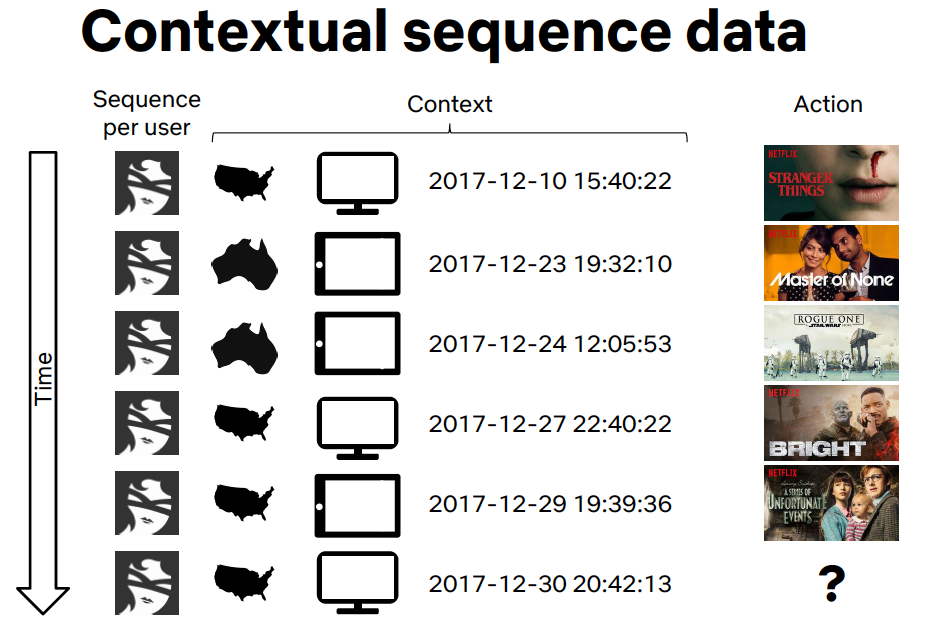
\includegraphics[width=0.7\textwidth]{assets/contextual-sequence-prediction.png}
    \caption[Context Filtering Diagram]{Context Filtering Diagram \cite{NvidiaRecSys}} 
\end{figure}
\subsection{Variational Autoencoder for Collaborative Filtering}
This model consists of two parts: an encoder and a decoder. The encoder takes the user's preferences as input and encodes them into a latent space. The decoder takes the latent space as input and decodes it into the item's features.
\begin{figure}[H]
    \centering
    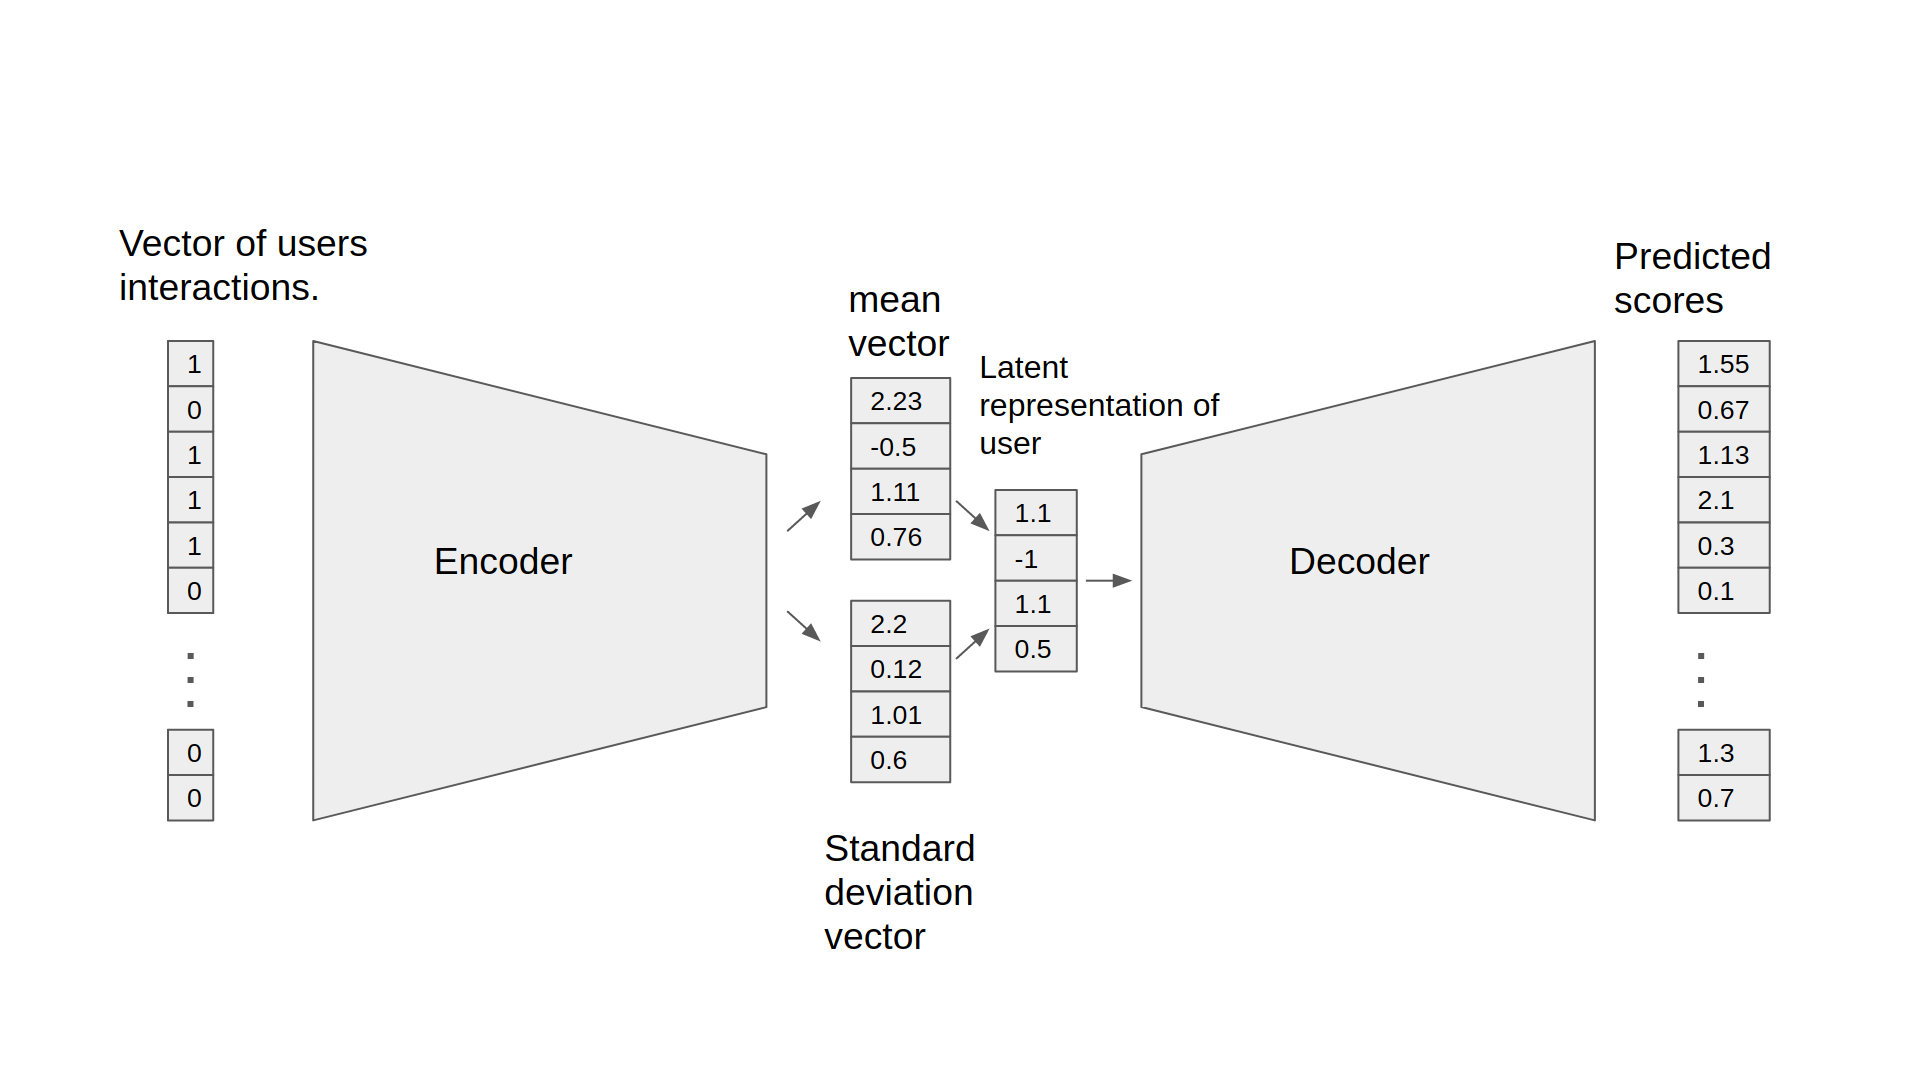
\includegraphics[width=0.7\textwidth]{assets/variational-autoencoder.png}
    \caption[Variational Autoencoder for Collaborative Filtering Structure]{Variational Autoencoder for Collaborative Filtering Structure \cite{NvidiaRecSys}}
    \label{fig:variational-autoencoder-for-collaborative-filtering}
\end{figure}
\subsection{Collaborative Filtering}
A technique that filters out products that a customer might like based on reactions by similar users. It functions by clustering customers into smaller sets with similar interests. Then it uses the items they show interest in to create a ranked suggestions list. The idea behind this technique is that individuals who have previously agreed will continue to do so in the future.
\subsection{Content Filtering}
A technique that uses the features of items a user has interacted with to recommend more items with similar features. This technique is based on the idea that if a customer shows interest in a particular product, he will also be interested in a similar product. \\



\begin{figure}[H]
    \centering
    \begin{subfigure}{.5\textwidth}
        \centering
        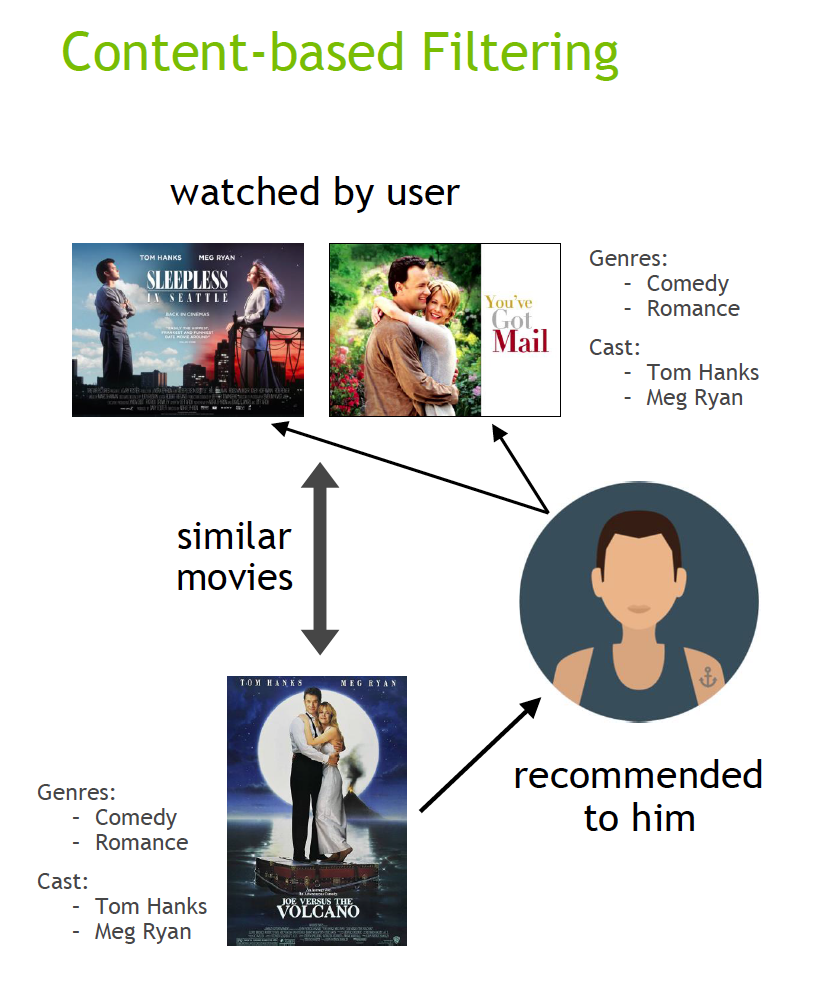
\includegraphics[width=0.8\linewidth]{assets/content_based_filtering.png}
        \caption{Content Filtering}
        \label{fig:content-filtering}
    \end{subfigure}%
    \begin{subfigure}{.5\textwidth}
        \centering
        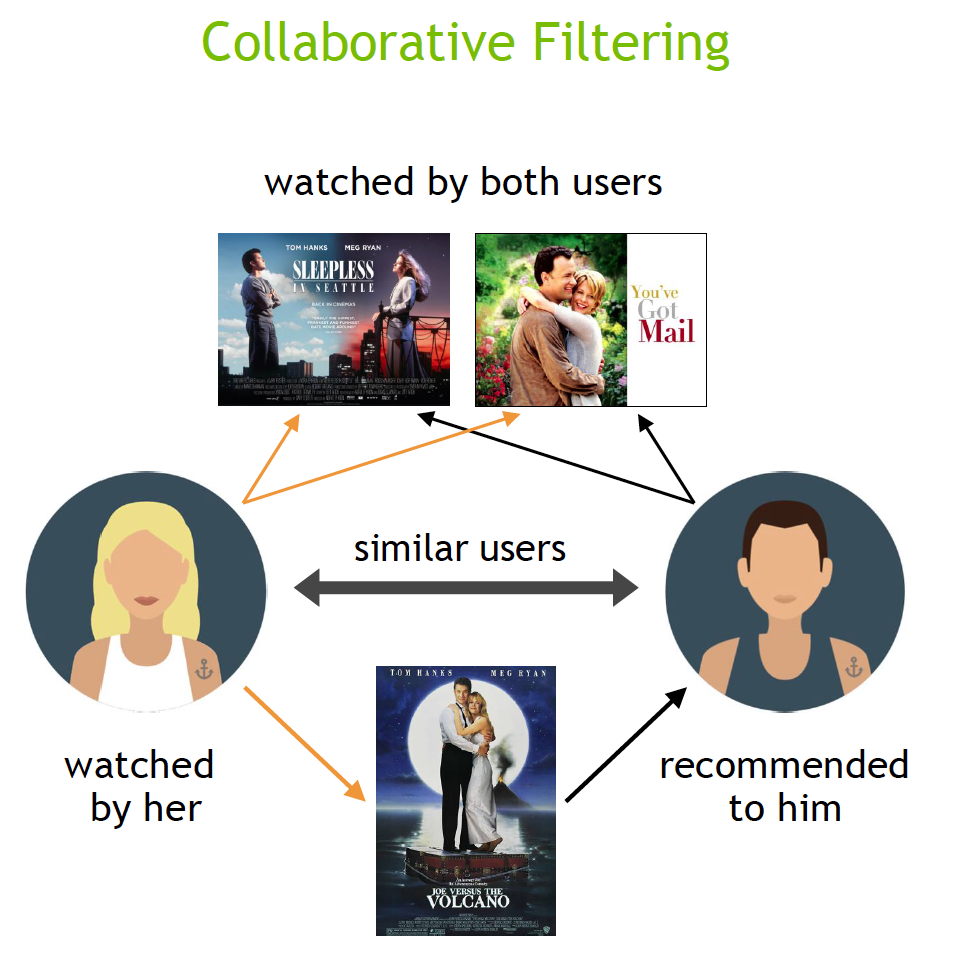
\includegraphics[width=0.95\linewidth]{assets/collaborative_filtering.png}
        \caption{Collaborative Filtering Diagram}
        \label{fig:collaborative-filtering}
    \end{subfigure}
    \caption[Nvidia Glossary Diagram]{Nvidia Glossary Diagram \cite{NvidiaRecSys}}
\end{figure}


\subsection{Hybrid Recommendation Systems}
Combine the advantages of multiple types of recommendation algorithms to create a more comprehensive recommending system.
\subsection{Neural Collaborative Filtering}
NCF is a technique that uses neural networks to learn the customer's preferences and recommend items. It uses one neural network that learns the customer's preferences and another neural network that learns the item's features. The two networks are then combined to create a recommendation.
\begin{figure}[H]
    \centering
    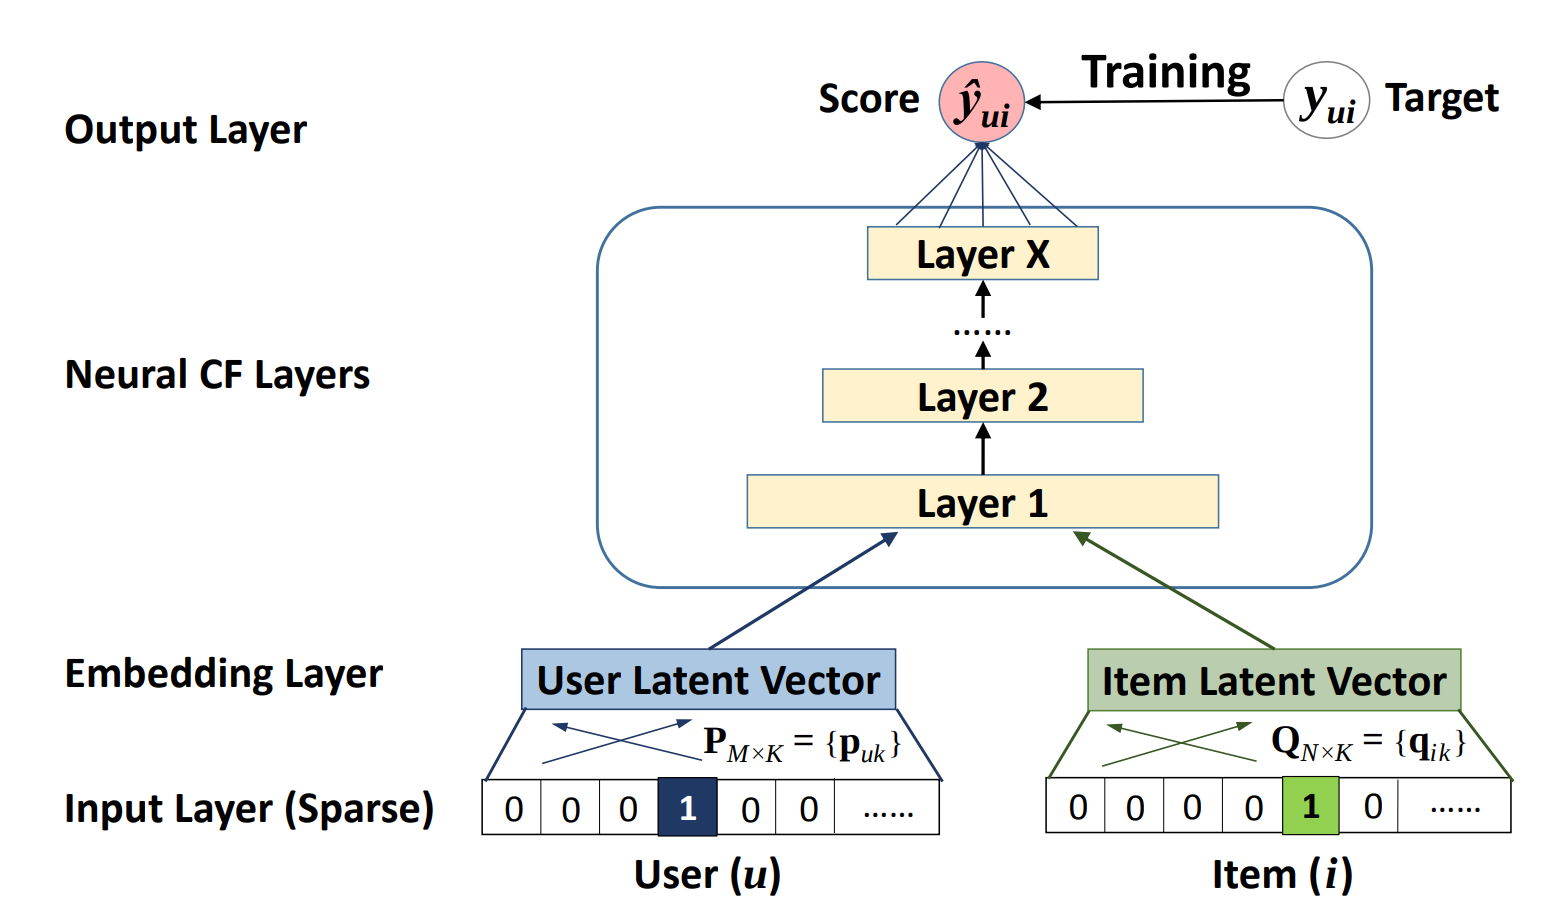
\includegraphics[width=0.8\textwidth]{assets/neural-collaborative-filtering.png}
    \caption[Neural Collaborative Filtering]{Neural Collaborative Filtering \cite{NvidiaRecSys}}
    \label{fig:neural-collaborative-filtering}
\end{figure}

\subsection{Contextual Sequence Learning}
Contextual Sequence Learning is a technique that takes into account the context and sequence of the user's action, it usually uses a recurrent neural network (RNN).
An example use case is session-based recommendations, RNNs predict the next items based on user event sequences, mirroring word embedding in NLP.
\subsection{Wide And Deep}
Wide \& Deep is a technique that uses a wide neural network to learn the preferences of the customer and utilizes another deep neural network to learn the products's features. The wide model is a generalized linear model (GLM) and the deep model is built from a dense neural network (DNN).
\begin{figure}[H]
    \centering
    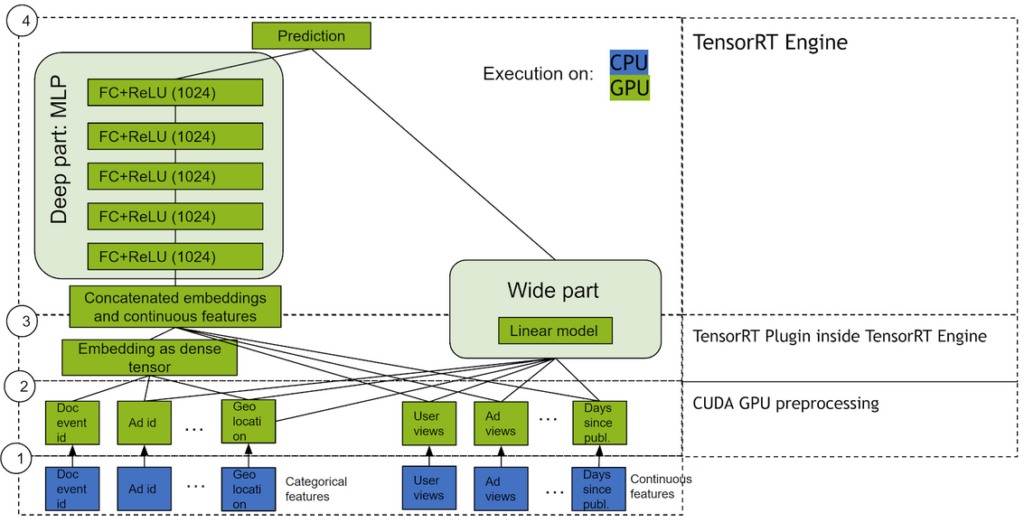
\includegraphics[width=0.8\textwidth]{assets/wide_deep.png}
    \caption[Wide Deep Structure]{Wide Deep Structure \cite{NvidiaRecSys}}
    \label{fig:wide-deep}
\end{figure}

\subsection{DLRM}
Deep Learning Recommendation Model (DLRM) is a technique that uses a deep neural network to handle categorical and numerical features. Each categorical feature is represented as a one-hot vector and each numerical feature is represented as a dense vector, both fed into multi-layer perceptron (MLP) layers. The output of the MLP layers is then fed into a dot product layer to compute the inner product of the feature vectors. The output of the dot product layer is then fed into a sigmoid layer to compute the probability of the user liking the item.
\begin{figure}[H]
    \centering
    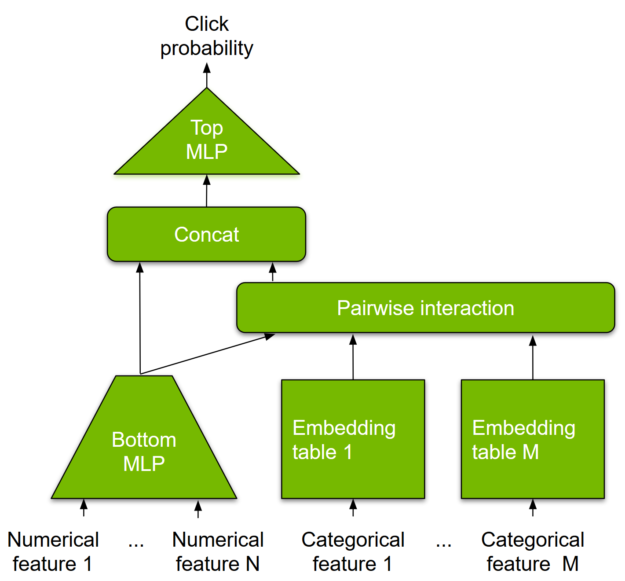
\includegraphics[width=0.7\textwidth]{assets/dlrm.png}
    \caption[DLRM Structure]{DLRM Structure \cite{NvidiaRecSys}}
    \label{fig:dlrm}
\end{figure}
